\documentclass{book}
\usepackage[a4paper,top=2.5cm,bottom=2.5cm,left=2.5cm,right=2.5cm]{geometry}
\usepackage{makeidx}
\usepackage{natbib}
\usepackage{graphicx}
\usepackage{multicol}
\usepackage{float}
\usepackage{listings}
\usepackage{color}
\usepackage{ifthen}
\usepackage[table]{xcolor}
\usepackage{textcomp}
\usepackage{alltt}
\usepackage{ifpdf}
\ifpdf
\usepackage[pdftex,
            pagebackref=true,
            colorlinks=true,
            linkcolor=blue,
            unicode
           ]{hyperref}
\else
\usepackage[ps2pdf,
            pagebackref=true,
            colorlinks=true,
            linkcolor=blue,
            unicode
           ]{hyperref}
\usepackage{pspicture}
\fi
\usepackage[utf8]{inputenc}
\usepackage{mathptmx}
\usepackage[scaled=.90]{helvet}
\usepackage{courier}
\usepackage{sectsty}
\usepackage{amssymb}
\usepackage[titles]{tocloft}
\usepackage{doxygen}
\lstset{language=C++,inputencoding=utf8,basicstyle=\footnotesize,breaklines=true,breakatwhitespace=true,tabsize=2,numbers=left }
\makeindex
\setcounter{tocdepth}{3}
\renewcommand{\footrulewidth}{0.4pt}
\renewcommand{\familydefault}{\sfdefault}
\hfuzz=15pt
\setlength{\emergencystretch}{15pt}
\hbadness=750
\tolerance=750
\begin{document}
\hypersetup{pageanchor=false,citecolor=blue}
\begin{titlepage}
\vspace*{7cm}
\begin{center}
{\Large P\-Redat\-Or2 \\[1ex]\large Sun Dec 9 2012 }\\
\vspace*{1cm}
{\large Generated by Doxygen 1.8.2}\\
\vspace*{0.5cm}
{\small Sun Dec 9 2012 15:22:35}\\
\end{center}
\end{titlepage}
\clearemptydoublepage
\pagenumbering{roman}
\tableofcontents
\clearemptydoublepage
\pagenumbering{arabic}
\hypersetup{pageanchor=true,citecolor=blue}
\chapter{Class Index}
\section{Class List}
Here are the classes, structs, unions and interfaces with brief descriptions\-:\begin{DoxyCompactList}
\item\contentsline{section}{\hyperlink{class_grp_species}{Grp\-Species} \\*Represents the Group of \hyperlink{class_species}{Species} – all the species that exist in the \hyperlink{class_world}{World} }{\pageref{class_grp_species}}{}
\item\contentsline{section}{\hyperlink{class_region}{Region} \\*Represents the \hyperlink{class_region}{Region} -\/ a territory where different species live }{\pageref{class_region}}{}
\item\contentsline{section}{\hyperlink{class_species}{Species} \\*Represents a base unit of the population – a \hyperlink{class_species}{Species} }{\pageref{class_species}}{}
\item\contentsline{section}{\hyperlink{class_world}{World} \\*Represents the \hyperlink{class_world}{World} – the group of Regions }{\pageref{class_world}}{}
\end{DoxyCompactList}

\chapter{File Index}
\section{File List}
Here is a list of all files with brief descriptions\-:\begin{DoxyCompactList}
\item\contentsline{section}{\hyperlink{_grp_species_8hpp}{Grp\-Species.\-hpp} \\*Specification of the \char`\"{}\-Grp\-Species\char`\"{} class }{\pageref{_grp_species_8hpp}}{}
\item\contentsline{section}{\hyperlink{pro2_8cpp}{pro2.\-cpp} }{\pageref{pro2_8cpp}}{}
\item\contentsline{section}{\hyperlink{_region_8hpp}{Region.\-hpp} \\*Specification of the \char`\"{}\-Region\char`\"{} class }{\pageref{_region_8hpp}}{}
\item\contentsline{section}{\hyperlink{_species_8hpp}{Species.\-hpp} \\*Specification of the \char`\"{}\-Species\char`\"{} class }{\pageref{_species_8hpp}}{}
\item\contentsline{section}{\hyperlink{_world_8hpp}{World.\-hpp} \\*Specification of the \char`\"{}\-World\char`\"{} class }{\pageref{_world_8hpp}}{}
\end{DoxyCompactList}

\chapter{Class Documentation}
\hypertarget{class_grp_species}{\section{Grp\-Species Class Reference}
\label{class_grp_species}\index{Grp\-Species@{Grp\-Species}}
}


Represents the Group of \hyperlink{class_species}{Species} – all the species that exist in the \hyperlink{class_world}{World}.  


\subsection*{Public Member Functions}
\begin{DoxyCompactItemize}
\item 
\hyperlink{class_grp_species_aae01eb441932fe90e69af5295f7449d3}{Grp\-Species} ()
\begin{DoxyCompactList}\small\item\em Default constructor. \end{DoxyCompactList}\item 
\hyperlink{class_grp_species_a528284319185c3d9e7dc23bdb6f47f58}{Grp\-Species} (vector$<$ \hyperlink{class_species}{Species} $>$ vspecies, vector$<$ int $>$ priority)
\begin{DoxyCompactList}\small\item\em Constructor with extended set of settings. \end{DoxyCompactList}\item 
\hyperlink{class_grp_species_aefa7f81cd9c5040080661a0aebbe94dd}{$\sim$\-Species} ()
\begin{DoxyCompactList}\small\item\em Default destructor. \end{DoxyCompactList}\item 
int \hyperlink{class_grp_species_ab7ed452e9d482a8f0a623ba0a4597fd1}{priority\-\_\-id} (int count)
\begin{DoxyCompactList}\small\item\em The consultor operation for the priority between species. \end{DoxyCompactList}\item 
int \hyperlink{class_grp_species_a6f8dd5cc59ac2647dead252ee64c8bd3}{priority\-\_\-size} ()
\begin{DoxyCompactList}\small\item\em Returns the size of the priority vector (the number of carnivorous species). \end{DoxyCompactList}\item 
bool \hyperlink{class_grp_species_a40bca706f2c7ff5c29ad64efef91f5b0}{is\-\_\-carnivorous} (int id)
\begin{DoxyCompactList}\small\item\em The member species carnivorousness consultor operation. \end{DoxyCompactList}\item 
int \hyperlink{class_grp_species_ad805d0ed7ae160591693a234cf13383e}{nutritious\-\_\-minimum} (int id)
\begin{DoxyCompactList}\small\item\em Nutritious minimum consultor operation. \end{DoxyCompactList}\item 
int \hyperlink{class_grp_species_ac1d5b1342c36aea055cc6bee2215f187}{nutritious\-\_\-value} (int id)
\begin{DoxyCompactList}\small\item\em Nutritious value consultor operation. \end{DoxyCompactList}\item 
void \hyperlink{class_grp_species_a5d5691f011fe8f195d3297f08a0596d7}{change\-\_\-prey\-\_\-preference} (int id)
\begin{DoxyCompactList}\small\item\em The operation of change of the prey vector. \end{DoxyCompactList}\item 
void \hyperlink{class_grp_species_acc72b9877cd8d59671a96762b51d87a1}{nprey} (int id)
\begin{DoxyCompactList}\small\item\em Returns the number of prey species for a species from the group. \end{DoxyCompactList}\item 
int \hyperlink{class_grp_species_ac486dcdf1d36b9935b396335f4567b6c}{prey\-\_\-id} (int id, int seq)
\begin{DoxyCompactList}\small\item\em The operation of consulting one of the possible prey species. \end{DoxyCompactList}\end{DoxyCompactItemize}


\subsection{Detailed Description}
Represents the Group of \hyperlink{class_species}{Species} – all the species that exist in the \hyperlink{class_world}{World}. 

Definition at line 13 of file Grp\-Species.\-hpp.



\subsection{Constructor \& Destructor Documentation}
\hypertarget{class_grp_species_aae01eb441932fe90e69af5295f7449d3}{\index{Grp\-Species@{Grp\-Species}!Grp\-Species@{Grp\-Species}}
\index{Grp\-Species@{Grp\-Species}!GrpSpecies@{Grp\-Species}}
\subsubsection[{Grp\-Species}]{\setlength{\rightskip}{0pt plus 5cm}Grp\-Species\-::\-Grp\-Species (
\begin{DoxyParamCaption}
{}
\end{DoxyParamCaption}
)}}\label{class_grp_species_aae01eb441932fe90e69af5295f7449d3}


Default constructor. 

Creates the empty group of species.

\begin{DoxyPrecond}{Precondition}
True. 
\end{DoxyPrecond}
\begin{DoxyPostcond}{Postcondition}
Implicit parameter is an empty instance if the \hyperlink{class_grp_species}{Grp\-Species} class. 
\end{DoxyPostcond}
\hypertarget{class_grp_species_a528284319185c3d9e7dc23bdb6f47f58}{\index{Grp\-Species@{Grp\-Species}!Grp\-Species@{Grp\-Species}}
\index{Grp\-Species@{Grp\-Species}!GrpSpecies@{Grp\-Species}}
\subsubsection[{Grp\-Species}]{\setlength{\rightskip}{0pt plus 5cm}Grp\-Species\-::\-Grp\-Species (
\begin{DoxyParamCaption}
\item[{vector$<$ {\bf Species} $>$}]{vspecies, }
\item[{vector$<$ int $>$}]{priority}
\end{DoxyParamCaption}
)}}\label{class_grp_species_a528284319185c3d9e7dc23bdb6f47f58}


Constructor with extended set of settings. 

Creates the group of species with the vector of \hyperlink{class_species}{Species} specified by the first explicit parameter and the priority between those species specified by the second explicit parameter.

\begin{DoxyPrecond}{Precondition}
True. 
\end{DoxyPrecond}
\begin{DoxyPostcond}{Postcondition}
The group of species with the member species specified by the explicit parameters is created. 
\end{DoxyPostcond}
\hypertarget{class_grp_species_aefa7f81cd9c5040080661a0aebbe94dd}{\index{Grp\-Species@{Grp\-Species}!$\sim$\-Species@{$\sim$\-Species}}
\index{$\sim$\-Species@{$\sim$\-Species}!GrpSpecies@{Grp\-Species}}
\subsubsection[{$\sim$\-Species}]{\setlength{\rightskip}{0pt plus 5cm}Grp\-Species\-::$\sim$\-Species (
\begin{DoxyParamCaption}
{}
\end{DoxyParamCaption}
)}}\label{class_grp_species_aefa7f81cd9c5040080661a0aebbe94dd}


Default destructor. 

Executed when the instance of \hyperlink{class_grp_species}{Grp\-Species} gets out of scope.

\begin{DoxyPrecond}{Precondition}
The implicit parameter is a \hyperlink{class_grp_species}{Grp\-Species} instance. 
\end{DoxyPrecond}
\begin{DoxyPostcond}{Postcondition}
The implicit parameter is destroyed. 
\end{DoxyPostcond}


\subsection{Member Function Documentation}
\hypertarget{class_grp_species_ab7ed452e9d482a8f0a623ba0a4597fd1}{\index{Grp\-Species@{Grp\-Species}!priority\-\_\-id@{priority\-\_\-id}}
\index{priority\-\_\-id@{priority\-\_\-id}!GrpSpecies@{Grp\-Species}}
\subsubsection[{priority\-\_\-id}]{\setlength{\rightskip}{0pt plus 5cm}int Grp\-Species\-::priority\-\_\-id (
\begin{DoxyParamCaption}
\item[{int}]{count}
\end{DoxyParamCaption}
)}}\label{class_grp_species_ab7ed452e9d482a8f0a623ba0a4597fd1}


The consultor operation for the priority between species. 

Allows us to get information about the priority in alimentation of the species of our group.

\begin{DoxyPrecond}{Precondition}
Implicit parameter is a valid group of species. Count is less than the total number of carnivorous species in the region and greater or equal than 0. 
\end{DoxyPrecond}
\begin{DoxyPostcond}{Postcondition}
The I\-D of the animal which has a priority of 'count' in the vector is returned. 
\end{DoxyPostcond}
\hypertarget{class_grp_species_a6f8dd5cc59ac2647dead252ee64c8bd3}{\index{Grp\-Species@{Grp\-Species}!priority\-\_\-size@{priority\-\_\-size}}
\index{priority\-\_\-size@{priority\-\_\-size}!GrpSpecies@{Grp\-Species}}
\subsubsection[{priority\-\_\-size}]{\setlength{\rightskip}{0pt plus 5cm}int Grp\-Species\-::priority\-\_\-size (
\begin{DoxyParamCaption}
{}
\end{DoxyParamCaption}
)}}\label{class_grp_species_a6f8dd5cc59ac2647dead252ee64c8bd3}


Returns the size of the priority vector (the number of carnivorous species). 

\begin{DoxyPrecond}{Precondition}
The implicit parameter is a valid group of species. 
\end{DoxyPrecond}
\begin{DoxyPostcond}{Postcondition}
The size of the priority vector is returned. 
\end{DoxyPostcond}
\hypertarget{class_grp_species_a40bca706f2c7ff5c29ad64efef91f5b0}{\index{Grp\-Species@{Grp\-Species}!is\-\_\-carnivorous@{is\-\_\-carnivorous}}
\index{is\-\_\-carnivorous@{is\-\_\-carnivorous}!GrpSpecies@{Grp\-Species}}
\subsubsection[{is\-\_\-carnivorous}]{\setlength{\rightskip}{0pt plus 5cm}bool Grp\-Species\-::is\-\_\-carnivorous (
\begin{DoxyParamCaption}
\item[{int}]{id}
\end{DoxyParamCaption}
)}}\label{class_grp_species_a40bca706f2c7ff5c29ad64efef91f5b0}


The member species carnivorousness consultor operation. 

Allows us to get the information about our species' carnivorousness.

\begin{DoxyPrecond}{Precondition}
The implicit parameter is a valid group of species. 

The animal with the specified id exists in our group of species. 
\end{DoxyPrecond}
\begin{DoxyPostcond}{Postcondition}
The information about the carnivorousness of the specified animal is returned. 
\end{DoxyPostcond}
\hypertarget{class_grp_species_ad805d0ed7ae160591693a234cf13383e}{\index{Grp\-Species@{Grp\-Species}!nutritious\-\_\-minimum@{nutritious\-\_\-minimum}}
\index{nutritious\-\_\-minimum@{nutritious\-\_\-minimum}!GrpSpecies@{Grp\-Species}}
\subsubsection[{nutritious\-\_\-minimum}]{\setlength{\rightskip}{0pt plus 5cm}int Grp\-Species\-::nutritious\-\_\-minimum (
\begin{DoxyParamCaption}
\item[{int}]{id}
\end{DoxyParamCaption}
)}}\label{class_grp_species_ad805d0ed7ae160591693a234cf13383e}


Nutritious minimum consultor operation. 

Allows us to get the nutritious minimum for the member species.

\begin{DoxyPrecond}{Precondition}
The implicit parameter is a valid group of species. 

The animal with the specified id exists in our group of species. 
\end{DoxyPrecond}
\begin{DoxyPostcond}{Postcondition}
The information about the nutritious minimum of the member species is returned. 
\end{DoxyPostcond}
\hypertarget{class_grp_species_ac1d5b1342c36aea055cc6bee2215f187}{\index{Grp\-Species@{Grp\-Species}!nutritious\-\_\-value@{nutritious\-\_\-value}}
\index{nutritious\-\_\-value@{nutritious\-\_\-value}!GrpSpecies@{Grp\-Species}}
\subsubsection[{nutritious\-\_\-value}]{\setlength{\rightskip}{0pt plus 5cm}int Grp\-Species\-::nutritious\-\_\-value (
\begin{DoxyParamCaption}
\item[{int}]{id}
\end{DoxyParamCaption}
)}}\label{class_grp_species_ac1d5b1342c36aea055cc6bee2215f187}


Nutritious value consultor operation. 

Allows us to get the nutritious value for the member species.

\begin{DoxyPrecond}{Precondition}
The implicit parameter is a valid group of species. 

The animal with the specified id exists in our group of species. 
\end{DoxyPrecond}
\begin{DoxyPostcond}{Postcondition}
The information about the nutritious value of the member species is returned. 
\end{DoxyPostcond}
\hypertarget{class_grp_species_a5d5691f011fe8f195d3297f08a0596d7}{\index{Grp\-Species@{Grp\-Species}!change\-\_\-prey\-\_\-preference@{change\-\_\-prey\-\_\-preference}}
\index{change\-\_\-prey\-\_\-preference@{change\-\_\-prey\-\_\-preference}!GrpSpecies@{Grp\-Species}}
\subsubsection[{change\-\_\-prey\-\_\-preference}]{\setlength{\rightskip}{0pt plus 5cm}void Grp\-Species\-::change\-\_\-prey\-\_\-preference (
\begin{DoxyParamCaption}
\item[{int}]{id}
\end{DoxyParamCaption}
)}}\label{class_grp_species_a5d5691f011fe8f195d3297f08a0596d7}


The operation of change of the prey vector. 

Allows us to update the prey preference for the the member species.

\begin{DoxyPrecond}{Precondition}
The implicit parameter is a valid group of species. 
\end{DoxyPrecond}
\begin{DoxyPostcond}{Postcondition}
The information about the updated prey preference is written to the prey vector of the member species. 
\end{DoxyPostcond}
\hypertarget{class_grp_species_acc72b9877cd8d59671a96762b51d87a1}{\index{Grp\-Species@{Grp\-Species}!nprey@{nprey}}
\index{nprey@{nprey}!GrpSpecies@{Grp\-Species}}
\subsubsection[{nprey}]{\setlength{\rightskip}{0pt plus 5cm}void Grp\-Species\-::nprey (
\begin{DoxyParamCaption}
\item[{int}]{id}
\end{DoxyParamCaption}
)}}\label{class_grp_species_acc72b9877cd8d59671a96762b51d87a1}


Returns the number of prey species for a species from the group. 

The operation that allows us to get the number of prey species for the animals of current group.

\begin{DoxyPrecond}{Precondition}
The id is greater or equal than 0 and less than the number of species of current group. 
\end{DoxyPrecond}
\begin{DoxyPostcond}{Postcondition}
The number of prey species for the 'id' species of current group is returned. 
\end{DoxyPostcond}
\hypertarget{class_grp_species_ac486dcdf1d36b9935b396335f4567b6c}{\index{Grp\-Species@{Grp\-Species}!prey\-\_\-id@{prey\-\_\-id}}
\index{prey\-\_\-id@{prey\-\_\-id}!GrpSpecies@{Grp\-Species}}
\subsubsection[{prey\-\_\-id}]{\setlength{\rightskip}{0pt plus 5cm}int Grp\-Species\-::prey\-\_\-id (
\begin{DoxyParamCaption}
\item[{int}]{id, }
\item[{int}]{seq}
\end{DoxyParamCaption}
)}}\label{class_grp_species_ac486dcdf1d36b9935b396335f4567b6c}


The operation of consulting one of the possible prey species. 

Allows us to get an id of a species with which we can alimentate current member animal.

\begin{DoxyPrecond}{Precondition}
The implicit parameter is a valid group of species. 
\end{DoxyPrecond}
\begin{DoxyPostcond}{Postcondition}
The id of a prey unit, registered in the prey vector of current member species under the prey\mbox{[}seq\mbox{]} is returned if it exists. If the member species' prey\mbox{[}seq\mbox{]} does not exist, -\/1 is returned. 
\end{DoxyPostcond}


The documentation for this class was generated from the following file\-:\begin{DoxyCompactItemize}
\item 
\hyperlink{_grp_species_8hpp}{Grp\-Species.\-hpp}\end{DoxyCompactItemize}

\hypertarget{class_region}{\section{Region Class Reference}
\label{class_region}\index{Region@{Region}}
}


Represents the \hyperlink{class_region}{Region} -\/ a territory where different species live.  


\subsection*{Public Member Functions}
\begin{DoxyCompactItemize}
\item 
\hyperlink{class_region_aa8796c9b4ac95da7f7ca4f374673800c}{Region} ()
\begin{DoxyCompactList}\small\item\em Default constructor. \end{DoxyCompactList}\item 
\hyperlink{class_region_ad60199ea545e7ceb0bb1b88b8f0d43f8}{Region} (vector$<$ int $>$ population)
\begin{DoxyCompactList}\small\item\em The constructor which provides the non-\/empty population vector on creation. \end{DoxyCompactList}\item 
\hyperlink{class_region_a3c3670fff78f7511d156e3b2f0bc6266}{$\sim$\-Region} ()
\begin{DoxyCompactList}\small\item\em Default destructor. \end{DoxyCompactList}\item 
void \hyperlink{class_region_a8124ecd078406df4edfb92861c9511e8}{fight} ()
\begin{DoxyCompactList}\small\item\em Fight launching operation for the current region. \end{DoxyCompactList}\item 
void \hyperlink{class_region_af822042e4b63e01b87e483fbabf2987d}{increase\-\_\-population} (int m, int id)
\begin{DoxyCompactList}\small\item\em Increases the population of certain species in current region. \end{DoxyCompactList}\item 
void \hyperlink{class_region_a38a911f9e1034421fd3706064385e4c5}{decrease\-\_\-population} (int m, int id)
\begin{DoxyCompactList}\small\item\em Decreases the population of certain species in current region. \end{DoxyCompactList}\item 
vector$<$ int $>$ \hyperlink{class_region_a76c03f5cb2a0f9941c7b00bbff59e9cb}{get\-\_\-population} ()
\begin{DoxyCompactList}\small\item\em Population consultory operation. \end{DoxyCompactList}\end{DoxyCompactItemize}


\subsection{Detailed Description}
Represents the \hyperlink{class_region}{Region} -\/ a territory where different species live. 

Definition at line 14 of file Region.\-hpp.



\subsection{Constructor \& Destructor Documentation}
\hypertarget{class_region_aa8796c9b4ac95da7f7ca4f374673800c}{\index{Region@{Region}!Region@{Region}}
\index{Region@{Region}!Region@{Region}}
\subsubsection[{Region}]{\setlength{\rightskip}{0pt plus 5cm}Region\-::\-Region (
\begin{DoxyParamCaption}
{}
\end{DoxyParamCaption}
)}}\label{class_region_aa8796c9b4ac95da7f7ca4f374673800c}


Default constructor. 

Creates the empty region.

\begin{DoxyPrecond}{Precondition}
True. 
\end{DoxyPrecond}
\begin{DoxyPostcond}{Postcondition}
Implicit parameter is an empty instance if the \hyperlink{class_region}{Region} class. 
\end{DoxyPostcond}
\hypertarget{class_region_ad60199ea545e7ceb0bb1b88b8f0d43f8}{\index{Region@{Region}!Region@{Region}}
\index{Region@{Region}!Region@{Region}}
\subsubsection[{Region}]{\setlength{\rightskip}{0pt plus 5cm}Region\-::\-Region (
\begin{DoxyParamCaption}
\item[{vector$<$ int $>$}]{population}
\end{DoxyParamCaption}
)}}\label{class_region_ad60199ea545e7ceb0bb1b88b8f0d43f8}


The constructor which provides the non-\/empty population vector on creation. 

Creates the region with some population of different species in it.

\begin{DoxyPrecond}{Precondition}
The explicit parameter is a valid vector 'animal id -\/ population'. 
\end{DoxyPrecond}
\begin{DoxyPostcond}{Postcondition}
The implicit parameter is a valid region with the population specified the the first explicit parameter. 
\end{DoxyPostcond}
\hypertarget{class_region_a3c3670fff78f7511d156e3b2f0bc6266}{\index{Region@{Region}!$\sim$\-Region@{$\sim$\-Region}}
\index{$\sim$\-Region@{$\sim$\-Region}!Region@{Region}}
\subsubsection[{$\sim$\-Region}]{\setlength{\rightskip}{0pt plus 5cm}Region\-::$\sim$\-Region (
\begin{DoxyParamCaption}
{}
\end{DoxyParamCaption}
)}}\label{class_region_a3c3670fff78f7511d156e3b2f0bc6266}


Default destructor. 

Executed when the instance of \hyperlink{class_region}{Region} gets out of scope.

\begin{DoxyPrecond}{Precondition}
The implicit parameter is a \hyperlink{class_region}{Region} instance. 
\end{DoxyPrecond}
\begin{DoxyPostcond}{Postcondition}
The implicit parameter is destroyed. 
\end{DoxyPostcond}


\subsection{Member Function Documentation}
\hypertarget{class_region_a8124ecd078406df4edfb92861c9511e8}{\index{Region@{Region}!fight@{fight}}
\index{fight@{fight}!Region@{Region}}
\subsubsection[{fight}]{\setlength{\rightskip}{0pt plus 5cm}void Region\-::fight (
\begin{DoxyParamCaption}
{}
\end{DoxyParamCaption}
)}}\label{class_region_a8124ecd078406df4edfb92861c9511e8}


Fight launching operation for the current region. 

The operation that lets us launch the fight between the species of the current region. During the fight all the species in the region eat till reach of the alimentary minimum or, otherwise, pass away.

\begin{DoxyPrecond}{Precondition}
The implicit parameter is a valid instance of the \hyperlink{class_region}{Region} class with a non-\/empty population vector. 
\end{DoxyPrecond}
\begin{DoxyPostcond}{Postcondition}
The fight between species is launched. 
\end{DoxyPostcond}
\hypertarget{class_region_af822042e4b63e01b87e483fbabf2987d}{\index{Region@{Region}!increase\-\_\-population@{increase\-\_\-population}}
\index{increase\-\_\-population@{increase\-\_\-population}!Region@{Region}}
\subsubsection[{increase\-\_\-population}]{\setlength{\rightskip}{0pt plus 5cm}void Region\-::increase\-\_\-population (
\begin{DoxyParamCaption}
\item[{int}]{m, }
\item[{int}]{id}
\end{DoxyParamCaption}
)}}\label{class_region_af822042e4b63e01b87e483fbabf2987d}


Increases the population of certain species in current region. 

\begin{DoxyPrecond}{Precondition}
Implicit parameter is an instance of the \hyperlink{class_region}{Region} class. 
\end{DoxyPrecond}
\begin{DoxyPostcond}{Postcondition}
Implicit parameter's \char`\"{}id\char`\"{} species population is increased by m. 
\end{DoxyPostcond}
\hypertarget{class_region_a38a911f9e1034421fd3706064385e4c5}{\index{Region@{Region}!decrease\-\_\-population@{decrease\-\_\-population}}
\index{decrease\-\_\-population@{decrease\-\_\-population}!Region@{Region}}
\subsubsection[{decrease\-\_\-population}]{\setlength{\rightskip}{0pt plus 5cm}void Region\-::decrease\-\_\-population (
\begin{DoxyParamCaption}
\item[{int}]{m, }
\item[{int}]{id}
\end{DoxyParamCaption}
)}}\label{class_region_a38a911f9e1034421fd3706064385e4c5}


Decreases the population of certain species in current region. 

\begin{DoxyPrecond}{Precondition}
Implicit parameter is an instance of the \hyperlink{class_region}{Region} class. 
\end{DoxyPrecond}
\begin{DoxyPostcond}{Postcondition}
Implicit parameter's \char`\"{}id\char`\"{} species population is decreased by m. 
\end{DoxyPostcond}
\hypertarget{class_region_a76c03f5cb2a0f9941c7b00bbff59e9cb}{\index{Region@{Region}!get\-\_\-population@{get\-\_\-population}}
\index{get\-\_\-population@{get\-\_\-population}!Region@{Region}}
\subsubsection[{get\-\_\-population}]{\setlength{\rightskip}{0pt plus 5cm}vector$<$int$>$ Region\-::get\-\_\-population (
\begin{DoxyParamCaption}
{}
\end{DoxyParamCaption}
)}}\label{class_region_a76c03f5cb2a0f9941c7b00bbff59e9cb}


Population consultory operation. 

\begin{DoxyPrecond}{Precondition}
Implicit parameter is an instance of the \hyperlink{class_region}{Region} class. 
\end{DoxyPrecond}
\begin{DoxyPostcond}{Postcondition}
Implicit parameter's population is returned as a vector of animal id -\/ value pairs. 
\end{DoxyPostcond}


The documentation for this class was generated from the following file\-:\begin{DoxyCompactItemize}
\item 
\hyperlink{_region_8hpp}{Region.\-hpp}\end{DoxyCompactItemize}

\hypertarget{class_species}{\section{Species Class Reference}
\label{class_species}\index{Species@{Species}}
}


Represents a base unit of the population – a \hyperlink{class_species}{Species}.  


\subsection*{Public Member Functions}
\begin{DoxyCompactItemize}
\item 
\hyperlink{class_species_abb0f8e3208b0cc676157b7dff837c0be}{Species} ()
\begin{DoxyCompactList}\small\item\em Default constructor. \end{DoxyCompactList}\item 
\hyperlink{class_species_a16b8ced46ad340a73971735788c4da6e}{Species} (bool carnivorous, int nutritious\-\_\-minimum, int nutritious\-\_\-value, int nprey, vector$<$ int $>$ prey)
\begin{DoxyCompactList}\small\item\em Constructor with extended set of settings. \end{DoxyCompactList}\item 
\hyperlink{class_species_af36f93648e2dedc2f05b6fb0c067f35e}{$\sim$\-Species} ()
\begin{DoxyCompactList}\small\item\em Default destructor. \end{DoxyCompactList}\item 
bool \hyperlink{class_species_ae9693788c20d6ba84b8dd950f1e90296}{is\-\_\-carnivorous} ()
\begin{DoxyCompactList}\small\item\em Carnivorousness consultor operation. \end{DoxyCompactList}\item 
int \hyperlink{class_species_a1ff07d6d5a5d03978d2c8df16f49b8d7}{nutritious\-\_\-minimum} ()
\begin{DoxyCompactList}\small\item\em Nutritious minimum consultor operation. \end{DoxyCompactList}\item 
int \hyperlink{class_species_abea0a065bd95c118115b6647fccb87a0}{nutritious\-\_\-value} ()
\begin{DoxyCompactList}\small\item\em Nutritious value consultor operation. \end{DoxyCompactList}\item 
void \hyperlink{class_species_a1292192418e6b58ff78a539b3742f2fc}{change\-\_\-prey\-\_\-preference} ()
\begin{DoxyCompactList}\small\item\em The operation of change of the prey vector. \end{DoxyCompactList}\item 
int \hyperlink{class_species_a021f722194b0ce95c4f18de963f85a20}{prey\-\_\-id} (int seq)
\begin{DoxyCompactList}\small\item\em The operation of consulting one of the possible prey species. \end{DoxyCompactList}\item 
int \hyperlink{class_species_ab0efdbab578ade0701d39aa1ef7686fd}{nprey} ()
\begin{DoxyCompactList}\small\item\em The operation of consulting the number of the prey animals. \end{DoxyCompactList}\end{DoxyCompactItemize}


\subsection{Detailed Description}
Represents a base unit of the population – a \hyperlink{class_species}{Species}. 

Definition at line 12 of file Species.\-hpp.



\subsection{Constructor \& Destructor Documentation}
\hypertarget{class_species_abb0f8e3208b0cc676157b7dff837c0be}{\index{Species@{Species}!Species@{Species}}
\index{Species@{Species}!Species@{Species}}
\subsubsection[{Species}]{\setlength{\rightskip}{0pt plus 5cm}Species\-::\-Species (
\begin{DoxyParamCaption}
{}
\end{DoxyParamCaption}
)}}\label{class_species_abb0f8e3208b0cc676157b7dff837c0be}


Default constructor. 

Creates the empty species.

\begin{DoxyPrecond}{Precondition}
True. 
\end{DoxyPrecond}
\begin{DoxyPostcond}{Postcondition}
Implicit parameter is an empty instance if the \hyperlink{class_species}{Species} class. 
\end{DoxyPostcond}
\hypertarget{class_species_a16b8ced46ad340a73971735788c4da6e}{\index{Species@{Species}!Species@{Species}}
\index{Species@{Species}!Species@{Species}}
\subsubsection[{Species}]{\setlength{\rightskip}{0pt plus 5cm}Species\-::\-Species (
\begin{DoxyParamCaption}
\item[{bool}]{carnivorous, }
\item[{int}]{nutritious\-\_\-minimum, }
\item[{int}]{nutritious\-\_\-value, }
\item[{int}]{nprey, }
\item[{vector$<$ int $>$}]{prey}
\end{DoxyParamCaption}
)}}\label{class_species_a16b8ced46ad340a73971735788c4da6e}


Constructor with extended set of settings. 

Creates the species with the specified values of carnivorousness, nutritious minimum, nutritious value, number of possible prey species and the vector of these prey species.

\begin{DoxyPrecond}{Precondition}
All the parameters have valid values. 
\end{DoxyPrecond}
\begin{DoxyPostcond}{Postcondition}
The species with all the necessary information is created. 
\end{DoxyPostcond}
\hypertarget{class_species_af36f93648e2dedc2f05b6fb0c067f35e}{\index{Species@{Species}!$\sim$\-Species@{$\sim$\-Species}}
\index{$\sim$\-Species@{$\sim$\-Species}!Species@{Species}}
\subsubsection[{$\sim$\-Species}]{\setlength{\rightskip}{0pt plus 5cm}Species\-::$\sim$\-Species (
\begin{DoxyParamCaption}
{}
\end{DoxyParamCaption}
)}}\label{class_species_af36f93648e2dedc2f05b6fb0c067f35e}


Default destructor. 

Executed when the instance of \hyperlink{class_species}{Species} gets out of scope.

\begin{DoxyPrecond}{Precondition}
The implicit parameter is a non-\/empty \hyperlink{class_species}{Species} instance. 
\end{DoxyPrecond}
\begin{DoxyPostcond}{Postcondition}
The implicit parameter is destroyed. 
\end{DoxyPostcond}


\subsection{Member Function Documentation}
\hypertarget{class_species_ae9693788c20d6ba84b8dd950f1e90296}{\index{Species@{Species}!is\-\_\-carnivorous@{is\-\_\-carnivorous}}
\index{is\-\_\-carnivorous@{is\-\_\-carnivorous}!Species@{Species}}
\subsubsection[{is\-\_\-carnivorous}]{\setlength{\rightskip}{0pt plus 5cm}bool Species\-::is\-\_\-carnivorous (
\begin{DoxyParamCaption}
{}
\end{DoxyParamCaption}
)}}\label{class_species_ae9693788c20d6ba84b8dd950f1e90296}


Carnivorousness consultor operation. 

Allows us to determine whether the species is carnivorous.

\begin{DoxyPrecond}{Precondition}
The implicit parameter is a valid instance of \hyperlink{class_species}{Species} class. 
\end{DoxyPrecond}
\begin{DoxyPostcond}{Postcondition}
The information about carnivorousness of the implicit parameter is returned. 
\end{DoxyPostcond}
\hypertarget{class_species_a1ff07d6d5a5d03978d2c8df16f49b8d7}{\index{Species@{Species}!nutritious\-\_\-minimum@{nutritious\-\_\-minimum}}
\index{nutritious\-\_\-minimum@{nutritious\-\_\-minimum}!Species@{Species}}
\subsubsection[{nutritious\-\_\-minimum}]{\setlength{\rightskip}{0pt plus 5cm}int Species\-::nutritious\-\_\-minimum (
\begin{DoxyParamCaption}
{}
\end{DoxyParamCaption}
)}}\label{class_species_a1ff07d6d5a5d03978d2c8df16f49b8d7}


Nutritious minimum consultor operation. 

Allows us to get the nutritious minimum for current species.

\begin{DoxyPrecond}{Precondition}
The implicit parameter is a valid instance of \hyperlink{class_species}{Species} class. 
\end{DoxyPrecond}
\begin{DoxyPostcond}{Postcondition}
The information about the nutritious minimum of the implicit parameter is returned. 
\end{DoxyPostcond}
\hypertarget{class_species_abea0a065bd95c118115b6647fccb87a0}{\index{Species@{Species}!nutritious\-\_\-value@{nutritious\-\_\-value}}
\index{nutritious\-\_\-value@{nutritious\-\_\-value}!Species@{Species}}
\subsubsection[{nutritious\-\_\-value}]{\setlength{\rightskip}{0pt plus 5cm}int Species\-::nutritious\-\_\-value (
\begin{DoxyParamCaption}
{}
\end{DoxyParamCaption}
)}}\label{class_species_abea0a065bd95c118115b6647fccb87a0}


Nutritious value consultor operation. 

Allows us to get the nutritious value for current species.

\begin{DoxyPrecond}{Precondition}
The implicit parameter is a valid instance of \hyperlink{class_species}{Species} class. 
\end{DoxyPrecond}
\begin{DoxyPostcond}{Postcondition}
The information about the nutritious value of the implicit parameter is returned. 
\end{DoxyPostcond}
\hypertarget{class_species_a1292192418e6b58ff78a539b3742f2fc}{\index{Species@{Species}!change\-\_\-prey\-\_\-preference@{change\-\_\-prey\-\_\-preference}}
\index{change\-\_\-prey\-\_\-preference@{change\-\_\-prey\-\_\-preference}!Species@{Species}}
\subsubsection[{change\-\_\-prey\-\_\-preference}]{\setlength{\rightskip}{0pt plus 5cm}void Species\-::change\-\_\-prey\-\_\-preference (
\begin{DoxyParamCaption}
{}
\end{DoxyParamCaption}
)}}\label{class_species_a1292192418e6b58ff78a539b3742f2fc}


The operation of change of the prey vector. 

Allows us to update the prey preference for the current species

\begin{DoxyPrecond}{Precondition}
The implicit parameter is a valid instance of \hyperlink{class_species}{Species} class. 
\end{DoxyPrecond}
\begin{DoxyPostcond}{Postcondition}
The information about the updated prey preference is written to the prey vector of the implicit parameter. 
\end{DoxyPostcond}
\hypertarget{class_species_a021f722194b0ce95c4f18de963f85a20}{\index{Species@{Species}!prey\-\_\-id@{prey\-\_\-id}}
\index{prey\-\_\-id@{prey\-\_\-id}!Species@{Species}}
\subsubsection[{prey\-\_\-id}]{\setlength{\rightskip}{0pt plus 5cm}int Species\-::prey\-\_\-id (
\begin{DoxyParamCaption}
\item[{int}]{seq}
\end{DoxyParamCaption}
)}}\label{class_species_a021f722194b0ce95c4f18de963f85a20}


The operation of consulting one of the possible prey species. 

Allows us to get an id of a species with which we can alimentate current animal.

\begin{DoxyPrecond}{Precondition}
The implicit parameter is a valid instance of \hyperlink{class_species}{Species} class. 
\end{DoxyPrecond}
\begin{DoxyPostcond}{Postcondition}
The id of a prey unit, registered in the prey vector of current species under the prey\mbox{[}seq\mbox{]} is returned if it exists. If the prey\mbox{[}seq\mbox{]} does not exist, -\/1 is returned. 
\end{DoxyPostcond}
\hypertarget{class_species_ab0efdbab578ade0701d39aa1ef7686fd}{\index{Species@{Species}!nprey@{nprey}}
\index{nprey@{nprey}!Species@{Species}}
\subsubsection[{nprey}]{\setlength{\rightskip}{0pt plus 5cm}int Species\-::nprey (
\begin{DoxyParamCaption}
{}
\end{DoxyParamCaption}
)}}\label{class_species_ab0efdbab578ade0701d39aa1ef7686fd}


The operation of consulting the number of the prey animals. 

\begin{DoxyPrecond}{Precondition}
The implicit parameter is a valid instance of \hyperlink{class_species}{Species} class. 
\end{DoxyPrecond}
\begin{DoxyPostcond}{Postcondition}
The number of prey animals for current species is returned. 
\end{DoxyPostcond}


The documentation for this class was generated from the following file\-:\begin{DoxyCompactItemize}
\item 
\hyperlink{_species_8hpp}{Species.\-hpp}\end{DoxyCompactItemize}

\hypertarget{class_world}{\section{World Class Reference}
\label{class_world}\index{World@{World}}
}


Represents the \hyperlink{class_world}{World} – the group of Regions.  


\subsection*{Public Member Functions}
\begin{DoxyCompactItemize}
\item 
\hyperlink{class_world_afa39d4e6f714a7a3691ac0c656f5e8a8}{World} ()
\begin{DoxyCompactList}\small\item\em Default constructor. \end{DoxyCompactList}\item 
\hyperlink{class_world_afd90f5be9f4c530419d66fd656f9de8d}{World} (Arbre$<$ int $>$ structure, vector$<$ \hyperlink{class_region}{Region} $>$ regions)
\begin{DoxyCompactList}\small\item\em Constructor with the main data structures (the structure tree and the vector of regions) passed as an explicit parameters. \end{DoxyCompactList}\item 
\hyperlink{class_world_a8c73fba541a5817fff65147ba47cd827}{$\sim$\-World} ()
\begin{DoxyCompactList}\small\item\em Default destructor. \end{DoxyCompactList}\item 
void \hyperlink{class_world_a60f792899e98b54682755748f2576700}{fight} ()
\begin{DoxyCompactList}\small\item\em Fire up the fight between the species in the world. \end{DoxyCompactList}\item 
void \hyperlink{class_world_a97f4a9b980d4e11790568b05909eb8a2}{print\-\_\-population} ()
\begin{DoxyCompactList}\small\item\em Print the information about the population of the world. \end{DoxyCompactList}\item 
void \hyperlink{class_world_ad94ae4dc6a06819bca7ce2e0966ce5ab}{migrate\-\_\-central} (int r, int h, int spec\-\_\-id, int g)
\begin{DoxyCompactList}\small\item\em Perform a migration to the direction of the central plantation. \end{DoxyCompactList}\item 
void \hyperlink{class_world_a75f296ca8a787b3a1546cae8ab52767d}{migrate\-\_\-periferic} (int r, int h, int spec\-\_\-id, int g)
\begin{DoxyCompactList}\small\item\em Perform a migration to the direction of the perifery. \end{DoxyCompactList}\item 
void \hyperlink{class_world_ab997580c732ba82aa3847d0b3ac51dcf}{increase\-\_\-population} (int reg\-\_\-id, int m, int spec\-\_\-id)
\begin{DoxyCompactList}\small\item\em Increase the population of a certain species in a certain region. \end{DoxyCompactList}\end{DoxyCompactItemize}


\subsection{Detailed Description}
Represents the \hyperlink{class_world}{World} – the group of Regions. 

Definition at line 15 of file World.\-hpp.



\subsection{Constructor \& Destructor Documentation}
\hypertarget{class_world_afa39d4e6f714a7a3691ac0c656f5e8a8}{\index{World@{World}!World@{World}}
\index{World@{World}!World@{World}}
\subsubsection[{World}]{\setlength{\rightskip}{0pt plus 5cm}World\-::\-World (
\begin{DoxyParamCaption}
{}
\end{DoxyParamCaption}
)}}\label{class_world_afa39d4e6f714a7a3691ac0c656f5e8a8}


Default constructor. 

Executed on the creation of the new world.

\begin{DoxyPrecond}{Precondition}
True. 
\end{DoxyPrecond}
\begin{DoxyPostcond}{Postcondition}
The result is an empty world. 
\end{DoxyPostcond}
\hypertarget{class_world_afd90f5be9f4c530419d66fd656f9de8d}{\index{World@{World}!World@{World}}
\index{World@{World}!World@{World}}
\subsubsection[{World}]{\setlength{\rightskip}{0pt plus 5cm}World\-::\-World (
\begin{DoxyParamCaption}
\item[{Arbre$<$ int $>$}]{structure, }
\item[{vector$<$ {\bf Region} $>$}]{regions}
\end{DoxyParamCaption}
)}}\label{class_world_afd90f5be9f4c530419d66fd656f9de8d}


Constructor with the main data structures (the structure tree and the vector of regions) passed as an explicit parameters. 

\begin{DoxyPrecond}{Precondition}
True. 
\end{DoxyPrecond}
\begin{DoxyPostcond}{Postcondition}
The result is a world with the structure of regions specified in the explicit parameters. 
\end{DoxyPostcond}
\hypertarget{class_world_a8c73fba541a5817fff65147ba47cd827}{\index{World@{World}!$\sim$\-World@{$\sim$\-World}}
\index{$\sim$\-World@{$\sim$\-World}!World@{World}}
\subsubsection[{$\sim$\-World}]{\setlength{\rightskip}{0pt plus 5cm}World\-::$\sim$\-World (
\begin{DoxyParamCaption}
{}
\end{DoxyParamCaption}
)}}\label{class_world_a8c73fba541a5817fff65147ba47cd827}


Default destructor. 

Executed when the instance of \hyperlink{class_world}{World} gets out of scope.

\begin{DoxyPrecond}{Precondition}
The implicit parameter is a non-\/empty \hyperlink{class_world}{World} instance. 
\end{DoxyPrecond}
\begin{DoxyPostcond}{Postcondition}
The implicit parameter is destroyed. 
\end{DoxyPostcond}


\subsection{Member Function Documentation}
\hypertarget{class_world_a60f792899e98b54682755748f2576700}{\index{World@{World}!fight@{fight}}
\index{fight@{fight}!World@{World}}
\subsubsection[{fight}]{\setlength{\rightskip}{0pt plus 5cm}void World\-::fight (
\begin{DoxyParamCaption}
{}
\end{DoxyParamCaption}
)}}\label{class_world_a60f792899e98b54682755748f2576700}


Fire up the fight between the species in the world. 

\begin{DoxyPrecond}{Precondition}
The implicit parameter is a \hyperlink{class_world}{World} instance. 
\end{DoxyPrecond}
\begin{DoxyPostcond}{Postcondition}
The fight between species is launched in every region of the world. 
\end{DoxyPostcond}
\hypertarget{class_world_a97f4a9b980d4e11790568b05909eb8a2}{\index{World@{World}!print\-\_\-population@{print\-\_\-population}}
\index{print\-\_\-population@{print\-\_\-population}!World@{World}}
\subsubsection[{print\-\_\-population}]{\setlength{\rightskip}{0pt plus 5cm}void World\-::print\-\_\-population (
\begin{DoxyParamCaption}
{}
\end{DoxyParamCaption}
)}}\label{class_world_a97f4a9b980d4e11790568b05909eb8a2}


Print the information about the population of the world. 

\begin{DoxyPrecond}{Precondition}
The implicit parameter is a \hyperlink{class_world}{World} instance. 
\end{DoxyPrecond}
\begin{DoxyPostcond}{Postcondition}
The information about the population of the implicit parameter is written to stdout. 
\end{DoxyPostcond}
\hypertarget{class_world_ad94ae4dc6a06819bca7ce2e0966ce5ab}{\index{World@{World}!migrate\-\_\-central@{migrate\-\_\-central}}
\index{migrate\-\_\-central@{migrate\-\_\-central}!World@{World}}
\subsubsection[{migrate\-\_\-central}]{\setlength{\rightskip}{0pt plus 5cm}void World\-::migrate\-\_\-central (
\begin{DoxyParamCaption}
\item[{int}]{r, }
\item[{int}]{h, }
\item[{int}]{spec\-\_\-id, }
\item[{int}]{g}
\end{DoxyParamCaption}
)}}\label{class_world_ad94ae4dc6a06819bca7ce2e0966ce5ab}


Perform a migration to the direction of the central plantation. 

\begin{DoxyPrecond}{Precondition}
The implicit parameter is a non-\/empty \hyperlink{class_world}{World} instance. 
\end{DoxyPrecond}
\begin{DoxyPostcond}{Postcondition}
The migration of h individuums of spec\-\_\-id species originating in the region r in the direction of the central plantation is performed in the implicit parameter. 
\end{DoxyPostcond}
\hypertarget{class_world_a75f296ca8a787b3a1546cae8ab52767d}{\index{World@{World}!migrate\-\_\-periferic@{migrate\-\_\-periferic}}
\index{migrate\-\_\-periferic@{migrate\-\_\-periferic}!World@{World}}
\subsubsection[{migrate\-\_\-periferic}]{\setlength{\rightskip}{0pt plus 5cm}void World\-::migrate\-\_\-periferic (
\begin{DoxyParamCaption}
\item[{int}]{r, }
\item[{int}]{h, }
\item[{int}]{spec\-\_\-id, }
\item[{int}]{g}
\end{DoxyParamCaption}
)}}\label{class_world_a75f296ca8a787b3a1546cae8ab52767d}


Perform a migration to the direction of the perifery. 

\begin{DoxyPrecond}{Precondition}
The implicit parameter is a non-\/empty \hyperlink{class_world}{World} instance. 
\end{DoxyPrecond}
\begin{DoxyPostcond}{Postcondition}
The migration of h individuums of spec\-\_\-id species originating in the region r in the direction of the perifery is performed in the implicit parameter. 
\end{DoxyPostcond}
\hypertarget{class_world_ab997580c732ba82aa3847d0b3ac51dcf}{\index{World@{World}!increase\-\_\-population@{increase\-\_\-population}}
\index{increase\-\_\-population@{increase\-\_\-population}!World@{World}}
\subsubsection[{increase\-\_\-population}]{\setlength{\rightskip}{0pt plus 5cm}void World\-::increase\-\_\-population (
\begin{DoxyParamCaption}
\item[{int}]{reg\-\_\-id, }
\item[{int}]{m, }
\item[{int}]{spec\-\_\-id}
\end{DoxyParamCaption}
)}}\label{class_world_ab997580c732ba82aa3847d0b3ac51dcf}


Increase the population of a certain species in a certain region. 

\begin{DoxyPrecond}{Precondition}
The implicit parameter is a non-\/empty \hyperlink{class_world}{World} instance. 
\end{DoxyPrecond}
\begin{DoxyPostcond}{Postcondition}
The population of the species 'spec\-\_\-id' in the region 'reg\-\_\-id' is increased by 'm'. 
\end{DoxyPostcond}


The documentation for this class was generated from the following file\-:\begin{DoxyCompactItemize}
\item 
\hyperlink{_world_8hpp}{World.\-hpp}\end{DoxyCompactItemize}

\chapter{File Documentation}
\hypertarget{_grp_species_8hpp}{\section{Grp\-Species.\-hpp File Reference}
\label{_grp_species_8hpp}\index{Grp\-Species.\-hpp@{Grp\-Species.\-hpp}}
}


Specification of the \char`\"{}\-Grp\-Species\char`\"{} class.  


Include dependency graph for Grp\-Species.\-hpp\-:\nopagebreak
\begin{figure}[H]
\begin{center}
\leavevmode
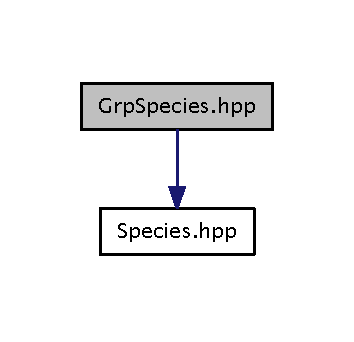
\includegraphics[width=236pt]{_grp_species_8hpp__incl}
\end{center}
\end{figure}
\subsection*{Classes}
\begin{DoxyCompactItemize}
\item 
class \hyperlink{class_grp_species}{Grp\-Species}
\begin{DoxyCompactList}\small\item\em Represents the Group of \hyperlink{class_species}{Species} – all the species that exist in the \hyperlink{class_world}{World}. \end{DoxyCompactList}\end{DoxyCompactItemize}


\subsection{Detailed Description}
Specification of the \char`\"{}\-Grp\-Species\char`\"{} class. 

Definition in file \hyperlink{_grp_species_8hpp_source}{Grp\-Species.\-hpp}.


\hypertarget{pro2_8cpp}{\section{pro2.\-cpp File Reference}
\label{pro2_8cpp}\index{pro2.\-cpp@{pro2.\-cpp}}
}
Include dependency graph for pro2.\-cpp\-:
\nopagebreak
\begin{figure}[H]
\begin{center}
\leavevmode
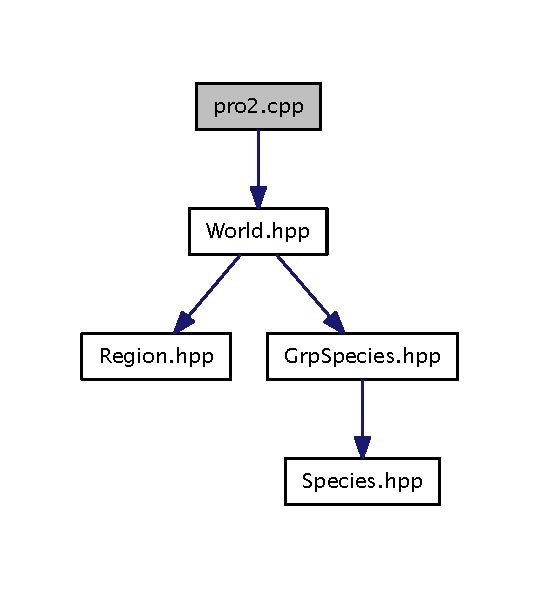
\includegraphics[width=259pt]{pro2_8cpp__incl}
\end{center}
\end{figure}
\subsection*{Functions}
\begin{DoxyCompactItemize}
\item 
void \hyperlink{pro2_8cpp_ad8853e739114a859d1e99d38abdc1cf3}{read\-\_\-tree} (Arbre$<$ int $>$ \&a, int marca)
\item 
int \hyperlink{pro2_8cpp_ae66f6b31b5ad750f1fe042a706a4e3d4}{main} ()
\end{DoxyCompactItemize}


\subsection{Function Documentation}
\hypertarget{pro2_8cpp_ad8853e739114a859d1e99d38abdc1cf3}{\index{pro2.\-cpp@{pro2.\-cpp}!read\-\_\-tree@{read\-\_\-tree}}
\index{read\-\_\-tree@{read\-\_\-tree}!pro2.cpp@{pro2.\-cpp}}
\subsubsection[{read\-\_\-tree}]{\setlength{\rightskip}{0pt plus 5cm}void read\-\_\-tree (
\begin{DoxyParamCaption}
\item[{Arbre$<$ int $>$ \&}]{a, }
\item[{int}]{marca}
\end{DoxyParamCaption}
)}}\label{pro2_8cpp_ad8853e739114a859d1e99d38abdc1cf3}


Definition at line 4 of file pro2.\-cpp.


\begin{DoxyCode}
                                         \{
    Arbre<int> a1;
    Arbre<int> a2;
    \textcolor{keywordtype}{int} x;
    cin >> x;
    \textcolor{keywordflow}{if} (x != marca) \{
        \hyperlink{pro2_8cpp_ad8853e739114a859d1e99d38abdc1cf3}{read\_tree}(a1, marca);
        \hyperlink{pro2_8cpp_ad8853e739114a859d1e99d38abdc1cf3}{read\_tree}(a2, marca);
        a.plantar(x,a1,a2);
    \}
\}
\end{DoxyCode}
\hypertarget{pro2_8cpp_ae66f6b31b5ad750f1fe042a706a4e3d4}{\index{pro2.\-cpp@{pro2.\-cpp}!main@{main}}
\index{main@{main}!pro2.cpp@{pro2.\-cpp}}
\subsubsection[{main}]{\setlength{\rightskip}{0pt plus 5cm}int main (
\begin{DoxyParamCaption}
{}
\end{DoxyParamCaption}
)}}\label{pro2_8cpp_ae66f6b31b5ad750f1fe042a706a4e3d4}


Definition at line 16 of file pro2.\-cpp.


\hypertarget{_region_8hpp}{\section{Region.\-hpp File Reference}
\label{_region_8hpp}\index{Region.\-hpp@{Region.\-hpp}}
}


Specification of the \char`\"{}\-Region\char`\"{} class.  


\subsection*{Classes}
\begin{DoxyCompactItemize}
\item 
class \hyperlink{class_region}{Region}
\begin{DoxyCompactList}\small\item\em Represents the \hyperlink{class_region}{Region} -\/ a territory where different species live. \end{DoxyCompactList}\end{DoxyCompactItemize}


\subsection{Detailed Description}
Specification of the \char`\"{}\-Region\char`\"{} class. 

Definition in file \hyperlink{_region_8hpp_source}{Region.\-hpp}.


\hypertarget{_species_8hpp}{\section{Species.\-hpp File Reference}
\label{_species_8hpp}\index{Species.\-hpp@{Species.\-hpp}}
}


Specification of the \char`\"{}\-Species\char`\"{} class.  


Include dependency graph for Species.\-hpp\-:\nopagebreak
\begin{figure}[H]
\begin{center}
\leavevmode
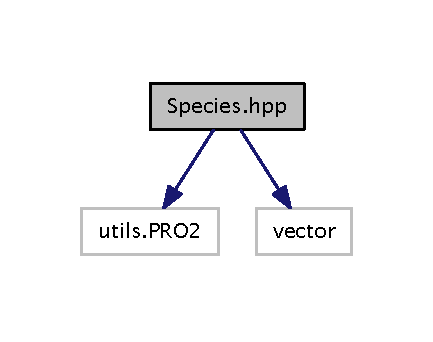
\includegraphics[width=208pt]{_species_8hpp__incl}
\end{center}
\end{figure}
\subsection*{Classes}
\begin{DoxyCompactItemize}
\item 
class \hyperlink{class_species}{Species}
\begin{DoxyCompactList}\small\item\em Represents a base unit of the population – a \hyperlink{class_species}{Species}. \end{DoxyCompactList}\end{DoxyCompactItemize}


\subsection{Detailed Description}
Specification of the \char`\"{}\-Species\char`\"{} class. 

Definition in file \hyperlink{_species_8hpp_source}{Species.\-hpp}.


\hypertarget{_world_8hpp}{\section{World.\-hpp File Reference}
\label{_world_8hpp}\index{World.\-hpp@{World.\-hpp}}
}


Specification of the \char`\"{}\-World\char`\"{} class.  


Include dependency graph for World.\-hpp\-:\nopagebreak
\begin{figure}[H]
\begin{center}
\leavevmode
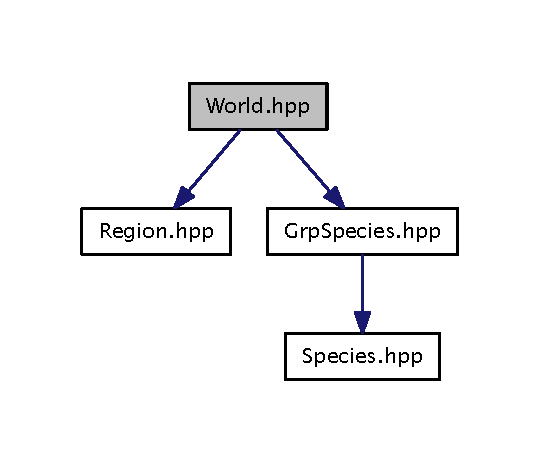
\includegraphics[width=283pt]{_world_8hpp__incl}
\end{center}
\end{figure}
\subsection*{Classes}
\begin{DoxyCompactItemize}
\item 
class \hyperlink{class_world}{World}
\begin{DoxyCompactList}\small\item\em Represents the \hyperlink{class_world}{World} – the group of Regions. \end{DoxyCompactList}\end{DoxyCompactItemize}


\subsection{Detailed Description}
Specification of the \char`\"{}\-World\char`\"{} class. 

Definition in file \hyperlink{_world_8hpp_source}{World.\-hpp}.


\addcontentsline{toc}{part}{Index}
\printindex
\end{document}
